\documentclass[12pt]{report}
\usepackage{geometry}                		% See geometry.pdf to learn the layout options. There are lots.
\geometry{letterpaper}                   		% ... or a4paper or a5paper or ... 
\usepackage{hyperref}
\usepackage{graphicx}				% Use pdf, png, jpg, or eps§ with pdflatex; use eps in DVI mode
\usepackage{fullpage}

\setlength{\parskip}{1em}
\author{Shiranka Miskin, Sam Maier, Dhruv Lal, William (Addison) Keizer \\ Source Code Here: https://github.com/SE2018-Capstone/shotsfired}
\title{Shots Fired - Architecture and Design}

\begin{document}
\maketitle

\tableofcontents
\chapter{Architecture}
\section{Challenges}

The main challenge that is shared amongst many games is that the complexity
involved is much higher than most other types of applications that may only need
to display information and handle simple interactivity.  Games such as ours must
be able to handle multiple entities acting simultaneously, performing a variety
of different tasks such as movement, performing actions like firing weapons, and
having other entities be able to affect them such as being damaged.  Inputs
through potentially multiple devices must be constantly polled and applied, and
the game must be continually drawn and updated.

This complexity is increased by a large factor when online
multiplayer is added. Now a single game must be synchronized between machines
despite the significant delay between updates due to having to transmit data
over an internet connection.  Significant effort was put into attempting
different ways of dealing with this latency.

Another challenge that applies to games more than it does to other applications
is performance.  The entire game must be able to process the inputs, update the
game, and display its results at a sufficient framerate to appear smooth to
users, the standard target framerate being 60 frames per second.

\section{Final Architecture}
\subsection{Client/Server}
There are multiple ways of solving the issue of synchronizing a game between
multiple computers (which will be referred to as "clients") over a network.  The
differences lie in what type of data is being transmitted from each client, and
which machine has "authority" about what the true state of the game is.

In Shots Fired, the server runs an entire copy of the game, which allows it to
act as the "source of truth" to keep all clients in sync.  The only information
that clients send to the server are their inputs, and then the server sends a
master copy of the game state to all the clients.  This allows for two very
important benefits, but has serious implications on the code.  To understand the
benefits, consider a scenario where the server did not have to run the game
logic, and it was only ran on the clients:  
\begin{enumerate}
    \item There is now the question of what the "true" state of the game is.
        Due to latency being in the hundreds of miliseconds, there is no
        guarantee that each client will process the game in exactly the same
        way.  Small differences in each client's state can result in a
        "butterfly effect", where each successive change simply increases just
        how desynchronized the clients are.  A way to get around this while
        still avoiding having to run the game on the server is to have one
        computer act as the host, and their state is taken to be the true state
        of the game.  The issue that arises here is the concept of "host
        advantage", where the player acting as a host now has 0 latency, while
        all other players have hundreds of miliseconds of latency.  
    \item Since the clients are given a measure of authority on the game state,
        it now becomes much easier to hack our game.  In order to run on
        browsers, the game is written in JavaScript, which, due to it being a
        scripted language and the debuggers that come built in to browsers, is
        easier for a user to make changes to than with other environments.  A
        player could theoretically simply send events to say "eliminate all
        other players" and they would win.  This is impossible in our
        architecture, as the only valid messages the server can process are
        snapshots of user input, such as which buttons they are pressing.
\end{enumerate}

\subsection{Node.js and Typescript}
One of the most significant implications of having to run the game logic on both
the client and the server is that in order for the code to be shared, it must be
able to be run on both platforms.  Since the game runs on the browser it must
be ran on JavaScript, or a language which can compile to JavaScript.  The forces
our choice of server technology to be Node.js, which allows servers to be
developed using JavaScript.

Significant effort was made to attempt a concurrent architecture on the server,
however after numerous road blocks due to the details of Node, it was deemed
to be infeasible.  JavaScript as a language is designed to be single threaded,
and Node.js simply does not accomodate for communication and sharing between
processes.

Out of the many language options which compile to JavaScript, TypeScript was
chosen in order to gain the many benefits of static type checking.  Being able
to assert the types of objects was even more significant due to the use of the
blackboard pattern. 

\subsection{Blackboard}
In order to keep all clients in sync, the server must be able to send
sufficient information on the game state over a websocket connection to the
clients.  This data must therefore be serializable, and must be sent over at a fast
enough rate, ideally 60 ticks per second just like the client, as to not allow
discrepancies between clients to build up.  To accomodate this, Shots Fired
implements a Blackboard style, where the entirety of the game state is stored in
a single JavaScript object.  The server is then able to easily forward updates
to the clients by simply sending this JavaScript object over, no potentially
costly serialization or deserialization is necessary.

There were other benefits of this architectural decision to store the game state in a
single JavaScript object.  In order to have the client replace its state with
the same state as the server, all that is necessary is to replace the value of
the state variable in the client with the data received from the server.  Having
it be a plain JavaScript object is also a great aid when it comes to debugging,
as a simple \texttt{console.log(game)} call will output the entire object in an
interactive and easily viewable format in the browser's debug menu.  It becomes
incredibly simple to view the entire state of the app at some point in time and
be able to figure out the cause of the issue at hand. Using typescript for type enforcement
allowed us to implement the objects this way and still ensure code clarity. 

\subsection{Pipe and Filter}
Shots Fired involves multiple entities which need to undergo a various set of
changes every frame of the game.  To process these in a structured manner, a
pipe and filter approach was implemented.  These updates to a game were kept
in strictly separate stages in order to reduce coupling between these
functionalities.  The original game object would be passed through these stages
to determine the state of the game for the next frame. This was done using events
and will be discussed further in the design portion of this report.

%\subsection{Events}
%In a game such as this, each entity may have various ways of affecting other
%entities, such as a bullet damaging a character or two character colliding.  In
%order to handle this very large number of possible interactions, an event-based
%approach was selected. Game entities are not permitted to affect change in any
%other entities other than through events.  Once all individual updates are
%applied to every entity, the resulting events are applied afterwards in their
%own stage.  Entity interaction becomes strictly decoupled from any individual
%interactions such as simple movement physics.

\section{Diagrams}
\subsection{Overall Architecture}
Clients and server run same Game Logic \\
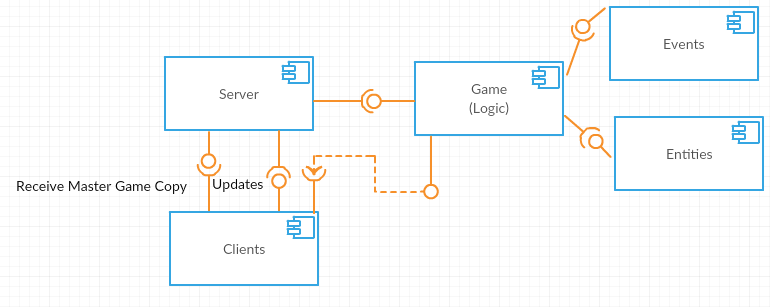
\includegraphics[width=\linewidth,height=5cm]{images/overall_architecture.png}

\subsection{Server Side Architecture}
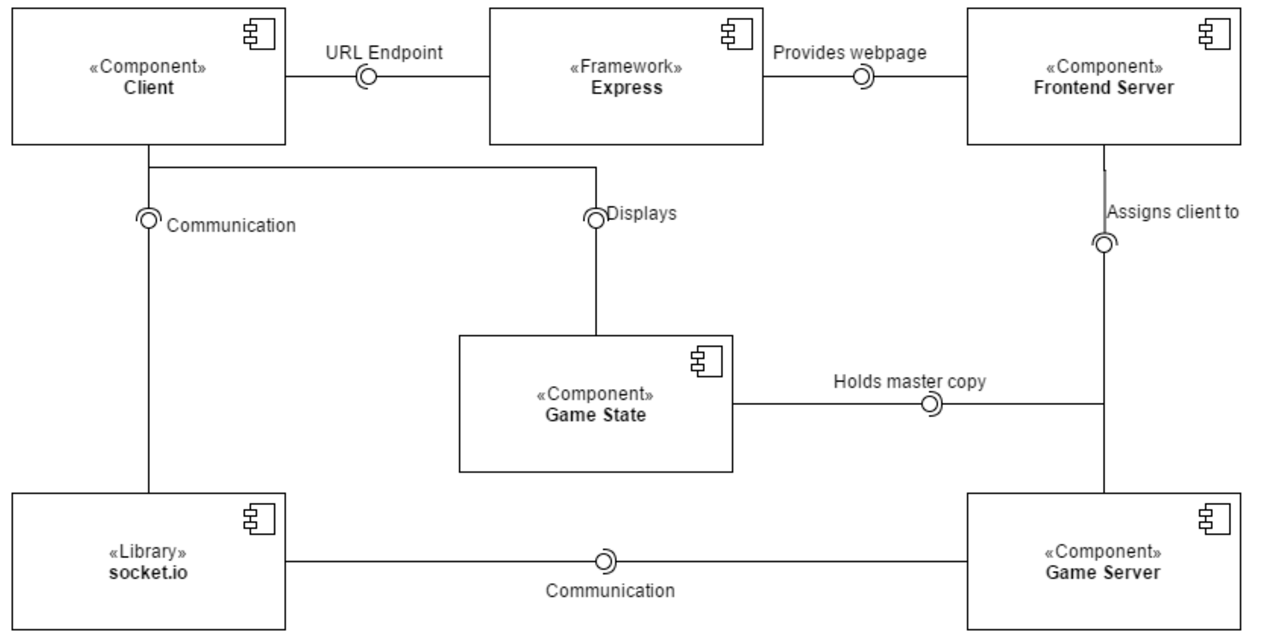
\includegraphics[width=\linewidth,height=7cm]{images/betterServerArchitecture.png}

\subsection{Client Side Architecture}
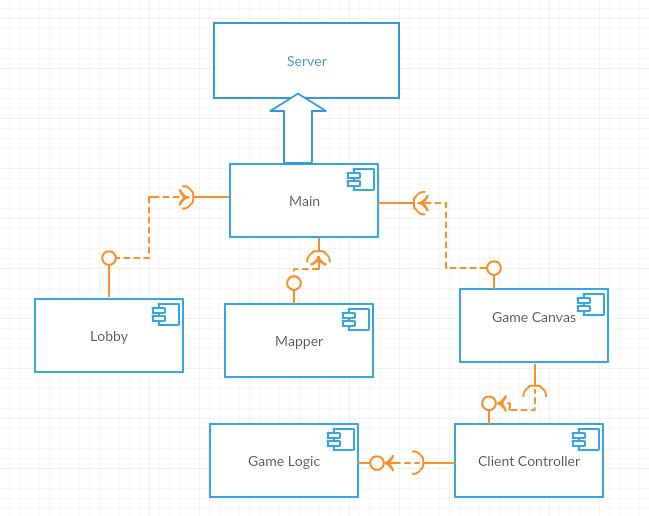
\includegraphics[width=\linewidth,height=7cm]{images/ClientArchitecture.png}

\subsection{Deployment Diagram}
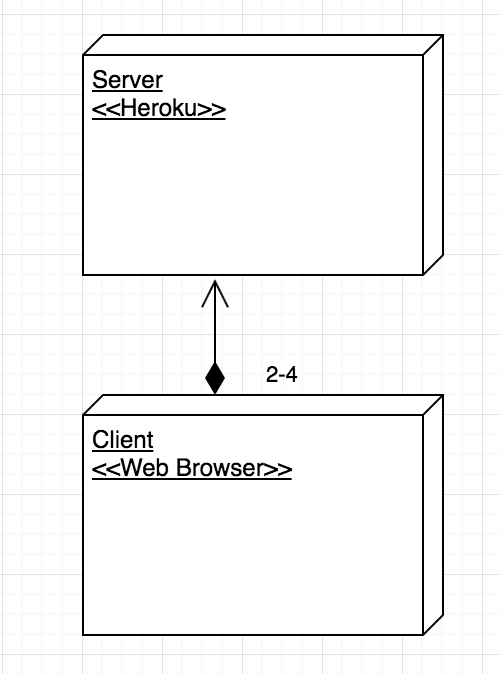
\includegraphics[height=7cm]{images/deploy_diagram.png}

\section{Requirements Results}
We were able to support the fundamentals of both of our functional and non functional requirements. 
\subsection{Functional Requirements}
The described architecture above results in a system which supports our Functional Requirements. Most of our functional requirements revolve around the implementation details of our system. The chosen architecture supports these by allowing or some computation to be done in the server, and some in the client. It allows for games to remain synced by the Blackboard pattern, and it uses a modified pipe and filter to implement game details.  
\subsection{Non-functional Attributes}
The chosen architecture allows us to satisfy our nonfunctional requirements. Our performance, when run locally, is quite smooth, and our method of sending inputs to the server and having the server send back the master state allowed this to work. We had some performance issues when running on Heroku, but the Heroku server has extremely variable ping which often gets quite high. This will severely impact any game. Within reason we therefore support the performance nonfunctional property. \\
Our game is easy to join due to our architecture allowing for the matchmaking system as well as the system to send a URL to friends to join a custom game. In addition since we implement this as a web application it is also very easy because a prospective user simply has to visit our website and click one button and they will be able to play a game. \\
The final two nonfunctional properties are not affected by architecture in particular, though we do support them nevertheless. Our game has a simple control scheme which satisfies the Simplicity nonfunctional property and we satisfied the Chrome 52+ requirement by ensuring we used supported javascript and polyfills if necessary in the build process.


\chapter{Design}

\section{Introduction}
Our application has three main sections. The server, the client, and the shared core functionality of the game. Each sections design will be discussed in turn in the design section of this document. A major part of the design in this application was our attempt to implement good Functional programming practices, whilst still using Design concepts from SE 464. Our emphasis on functional programming increases the coherence of our code, as most of our code is implement functionally.  
\section{Core -- Game Code}

The core code is found in the \texttt{src/core} folder. This is where the different game models and entities are contained. This code runs on both the client and the server. 


The \texttt{Game} model is found in the \texttt{game.ts} file, and is the main interface of the Game component in the architecture diagram. When created, it initializes an object of type \texttt{GameState}. This object will contain everything about the game 
%such as the game's settings like the minimum and maximum number of players, the list of players, the list of bullets, and a boolean which corresponds to whether the game is done or not. 
All of the methods within \texttt{Game} are used to modify a \texttt{GameState} variable given in the parameters. 
%These methods include \texttt{applyInputs}, \texttt{update} and \texttt{resolveEvents}. 
%They are called by the \texttt{ClientController}'s update function and this is whenever the previously mentioned \texttt{onTick} function is called in the \texttt{phaserUpdate()}. They are also called by the \texttt{GameServer} so that the server can update its copy of the game. 
The game display is updated at 60 fps. 

The \texttt{GameState} itself is a singleton on the client, but is an appropriate use of a singleton because it is necessary for the game to function for the game state to be a singleton. We do not want multiple representations of the game on a client, and there is no possible case for the future where this would happen. Each client will have its own, but the clients never directly interact.
It is necessary for the \texttt{GameState} to be a singleton on its machine because the server must be able to update the entire game state, and making it one central objects makes this very easy and efficient.

% The game implements the \textit{Mediator} design pattern. It does this through events. Game entities (see below), generate events. The entities do not change each other, they propagate these events to the \texttt{Game} system and the \texttt{Game} handles any changes necessary. This drastically decreases coupling in the application, by removing responsibility to make changes to entities to one interface (note that entities can still change themselves). 

%There is no need for multiple games on the same client. Furthermore internal to one GameInstance, there is no need for more then one game on the server. Having more would be unnecessary and would not happen. 

The \texttt{Entity} model is a very important class in the core. An \texttt{Entity} provides functions for anything that can be seen visually in the game like players, bullets and walls. This class contains base methods for updating \texttt{EntityState} objects. An \texttt{EntityState} contains information on the state of the entity. New Entity types should inherit from \texttt{Entity} for their class and \texttt{EntityState} for their data representation. This makes the game extensible since it is easy to add new entities into the game. The creation of a new data set (object) is done by a builder design pattern. The \texttt{Entity} class and its subclasses all define an \texttt{init()} function that is the builder function for the entity interface inheriting from \texttt{EntityState}. 

The \texttt{EntityState} interface family is a modified form of the Memento pattern.The internal state data is externalized as a data interface permanently. This allows us to represent the internal state as purely JSON data, so when we perform updates on the clients representation it is easy and efficient to restore the state to the current server decided state while simultaneously ensuring proper type checking. 

Entities, as a result single responsibility principle, can only modify a state of their own type. This leads to the necessity of handling interactions between entities. This is done through events in the  \texttt{event.ts} file. Events are created from the \texttt{EventFactory} and the interface for an \texttt{Event} object. This builder pattern, is used to generate an \texttt{Event} object containing necessary information which will be returned by an entity upon updating if necessary.

The \texttt{Game} class collects these events and reconciles all entities and ensure a coherent resultant game state. This is an example of the \textit{Mediator} design pattern. This drastically reduces coupling and increases coherence by making the computation sequential and ensuring that entities can only change their own type (Single Responsibility Principle). This part of the system is the Pipe and Filter architecture described above. 

Another design consideration was adhering to the Liskov Substitutability principle to ensure that when an State object that inherits from EntityState is used, an EntityState could also be used. This allows us greater reuse of methods. If more specific information is needed, those changes should happen inside the class that is the same type as the state.

Our system is very extensible. It can handle additions of any number of new game objects types. All it requires is adding a new state type and extending the correct classes. Alternate designs without the event system were considered. The event system was selected over not doing it to ensure an extensible system through reduced coupling. 

\subsection{Diagram of Entities}
This describes the inheritance relationship of the entities. It is easy to extend as you just have to inherit from entity.\\
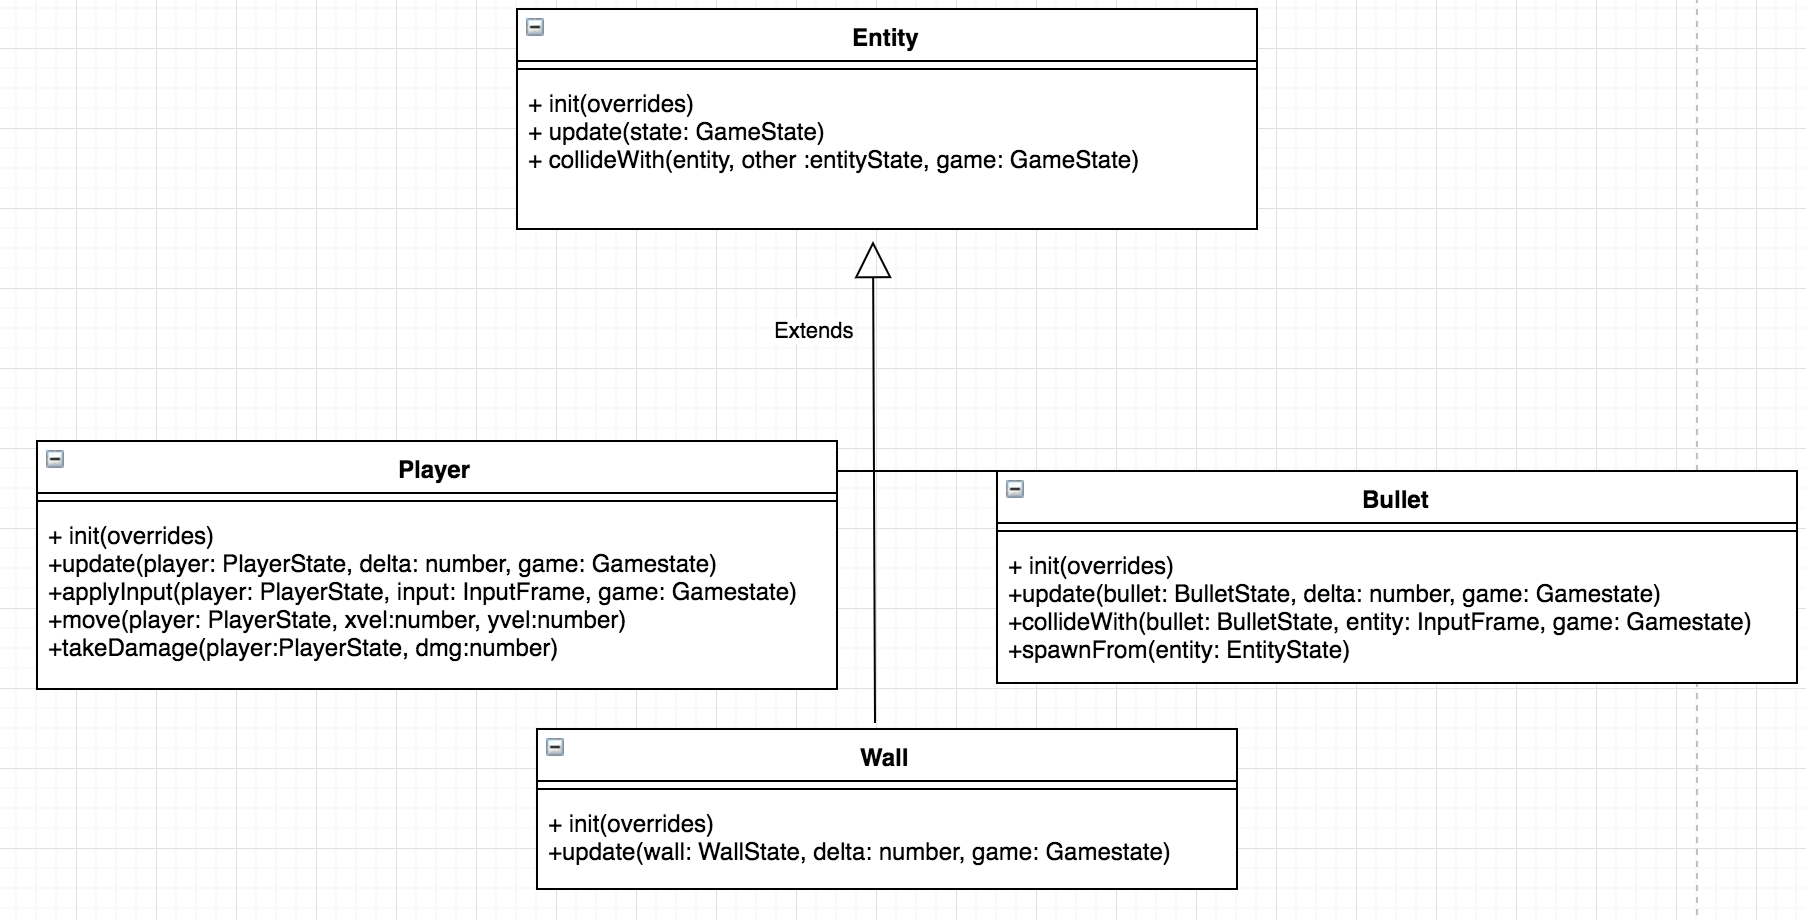
\includegraphics[width=\linewidth]{images/entities.png}

\subsection{State Relation Diagram}
Describes the Date Object interfaces used by the classes in Typescript. \\
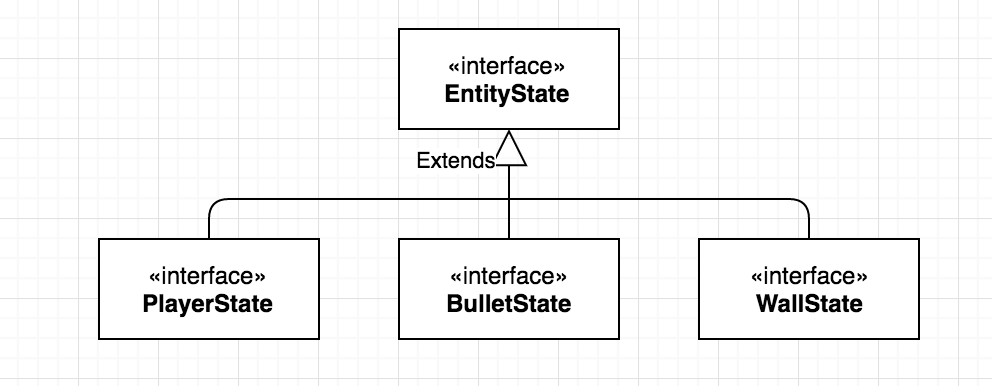
\includegraphics[width=\linewidth,height=5cm]{images/data_objects.png}


\section{Server}

The server's code is found in \texttt{src/server}. When we run \texttt{npm start}, we have a master server which is initialized in \texttt{server.ts}. This master server listens on some endpoints: \texttt{/}, which just serves our built frontend HTML and Javascript. \texttt{/join} and \texttt{/creategame} get forwarded to the \texttt{LobbyServer}, which provides the unique game URL to connect to. \texttt{/game/*} connects people to a specific game.
Games are uniquely identified by a randomly generated string of characters - one might look like \texttt{by6qp}. The \texttt{LobbyServer} performs the work of routing people to an appropriate game (assigning each player one of these strings of characters). It keeps track of the current lobby (in \texttt{currentRandLobby}), so that when people choose to join the quick play match, it knows which game to route to. Once 4 people have joined that lobby, it generates a new game identifier, and makes it the \texttt{currentRandLobby}. If only 2 or 3 people have joined, it starts a countdown, and if that countdown hits zero, it calls \texttt{startGame()} on its \texttt{GameServer}.


\texttt{GameServer} does not need to be 1:1 with \texttt{LobbyServer} - it was designed to be 1 \texttt{LobbyServer} to many \texttt{GameServers}, with each \texttt{GameServer} running on separate cores/machines to increase scalability and performance. We considered an alternate design where we used more concurrency, however, due to issues with Node.js's very restrictive multi-process API, we could not get multiple \texttt{GameServers} running across different cores.


\texttt{SocketIO::Socket} is a library class from SocketIO that we use for live communication from the server to the client. Each \texttt{GameInstance} stores 2-4 socket connections that is uses to communicate with the players.


Each \texttt{GameServer} has some number of \texttt{GameInstances}. It spins up a new one whenever a new game ID is requested. This \texttt{GameInstance} keeps its own  \texttt{Core::GameState} model as well as a buffer of \texttt{Core::InputFrames}. When players send new \texttt{Core::InputFrames} to the server, it buffers the \texttt{Core::InputFrames} until it can apply them on its master copy of the server. It then periodically resends its master copy of \texttt{Core::GameState} to the clients. It treats everything in \texttt{Core} as a complete black box - we just get these objects call \texttt{Core::InputFrame}, we apply them to another object called \texttt{Core::GameInstance}, and send the resulting \texttt{GameInstance} to the clients.

We use the Mediator design pattern where \texttt{GameInstance} acts as a Mediator between the GameServer and the Clients. This allows for easy extensibility as the GameServer does not need do know specific details about each instance, and therefore the GameInstance can handle the updates to the client. This makes our system easily extensible because it separates the handling of the clients from the handling of the Game backend. 

We also use an Observer pattern in the server to track events. This is necessary because in the server, requests happen asynchronously and we need to keep track events happening in the games and update our internal models accordingly. Essentially every time a client calls update, the server receives a notify that the state has changed and it can go retrieve the information to generate the new state. 

\subsection{Server Class Diagram}
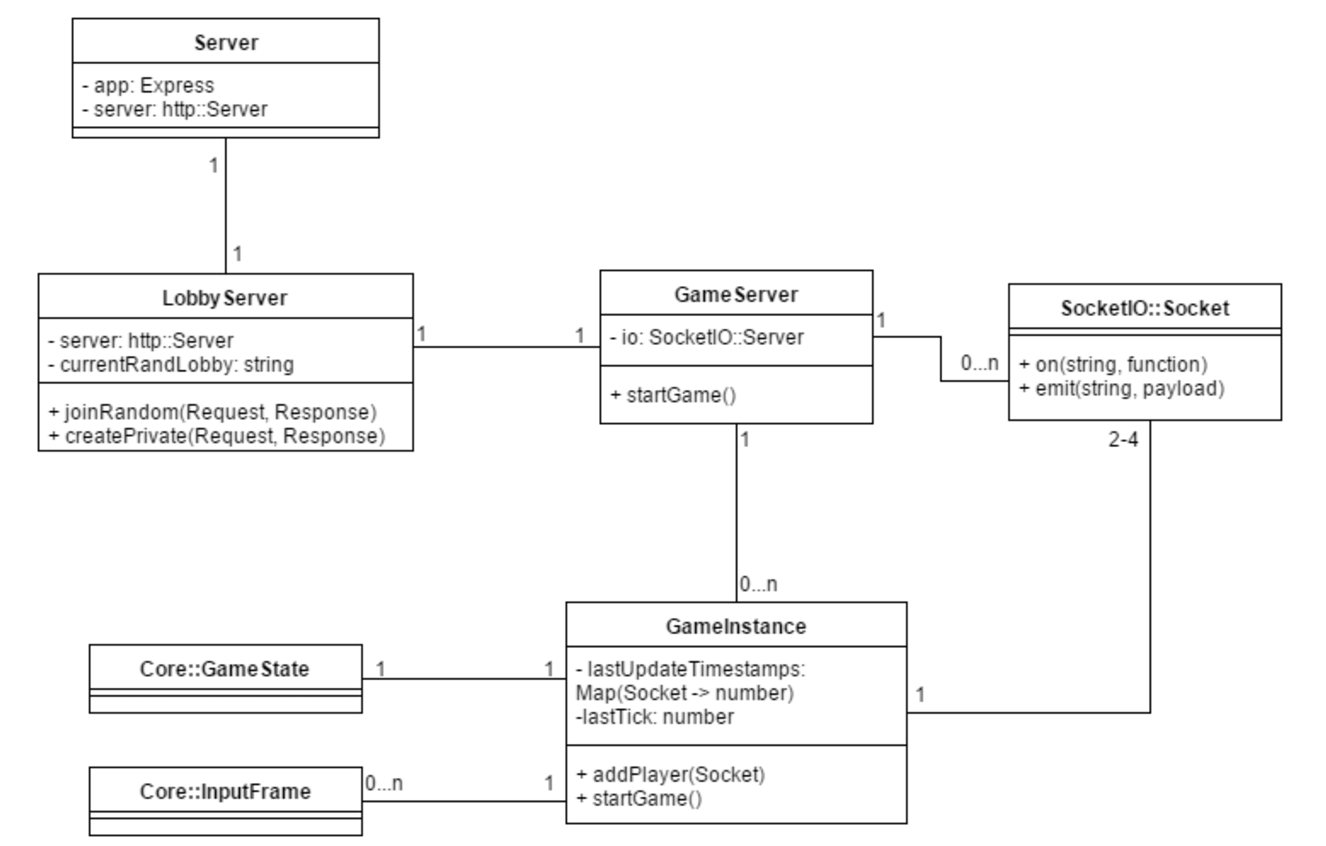
\includegraphics[width=\linewidth]{images/server_classes.png}

\section{Client}

The client code is found in \texttt{src/client}. Our system is structured similar to the MVP design pattern, where we have the view (our UI Client code), a ClientController class that operates the interaction between the backend and the UI and also controls the local game code (the presenter). The model can be seen as the "true state" server that fixes what our local game state simulates. This allows us to easily separate the UI code from the Control code, allowing for a more robust code system. 

The view is run with React.js and uses their standard system of including HTML code as XML style markup in display classes. the \texttt{main.tsx} file handles the upper level will load different pages that may need to be loaded. Primary pages that may be loaded include the Lobby, and Game system. To display the game, the UI uses a library called Phaser, which is used by the UI to display sprites, and handle react updates. Using this UI handler allowed us to focus on the multiplayer and game mechanic architecture. 

The ClientController, is essentially the presenter in the MVP pattern. It has responsibility to run the local copy of the game state, one model, and interface with the master copy on the server, another model. It propagates updates back to the presenter, which is the UI layer that implements Phaser. 

This implementation is has low coupling due to the separation of concerns and single responsibility principle of the MVP pattern, whereby the separation in to "View" and "Presenter" logic allows independent coding of display and functional requirements. 

Alternatives without the MVP style design were considered, but discarded due to the difficulty in ensuring enough separation from the game logic to allow it to run on both the client and server. 

\subsection{Architecture}
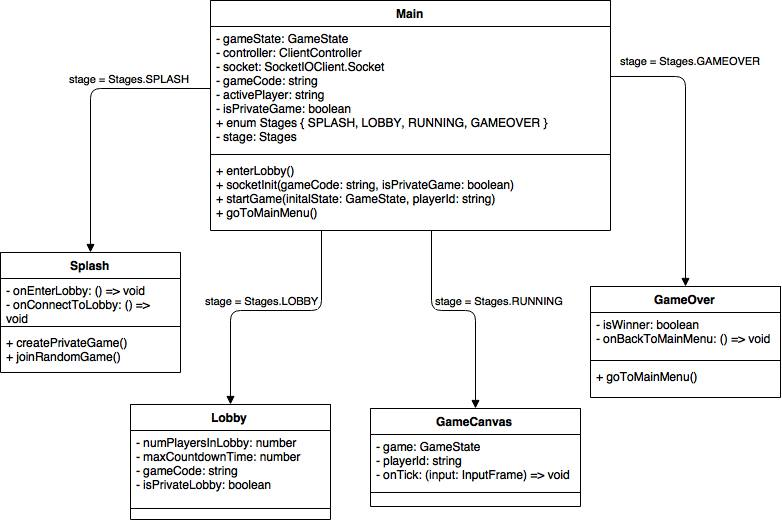
\includegraphics[width=\linewidth]{images/client_arch.png}
%Here we have the code for the client UI as well as the controller which the client uses to communicate with the server. The file \texttt{main.tsx} acts as the state manager. Depending on the state, a different component will be rendered for the client's display. The game starts out in the \texttt{SPLASH} state.


%The initial component is the \texttt{Splash} component. This component takes as input a function to connect to the lobby (\texttt{onConnectToLobby}) as well as a function to enter the lobby (\texttt{onEnterLobby}). This is the screen that contains the main menu. Here we see the name of the game, a brief description of the two game modes (Quick Play and Private Match), as well as the buttons to enter the lobbies for these game modes. When one of these buttons are clicked, the program will then either cause to user to join a random lobby, or allow them to make a private lobby that is only accessible to them. The state of \texttt{Main} gets changed to \texttt{LOBBY} regardless of the choice.


%Once in the \texttt{LOBBY} state, the component on display is \texttt{Lobby}. This component takes in the number of players in the lobby, the starting countdown time, the game code for the specific lobby as well as whether this lobby is private or not. There are represented by the parameters: \texttt{numPlayersInLobby}, \texttt{maxCountdownTime}, \texttt{gameCode}, and \texttt{isPrivateLobby} respectively. Here, a message is displayed to the user saying that you are waiting for more players to join. Once two or more people have entered the lobby, a countdown starts with \texttt{maxCountdownTime = 5000} milliseconds, which is displayed in seconds. As mentioned in the server section, once the countdown runs out or the maximum number of people have joined, the game will start. The state in \texttt{Main} changes to \texttt{RUNNING}.


%In this state, the \texttt{GameCanvas} component is now rendering. This component takes the game state, player ID and a periodic function that executes to update the game on the server, as input. These are given by the parameters: \texttt{game}, \texttt{playerId} and \texttt{onTick} respectively. \texttt{GameCanvas} is primarily Phaser based meaning that it contains functions that will allow it to re-render/update itself without anyone else telling the component to update. This is made possible by the \texttt{phaserPreload()}, \texttt{phaserCreate()}, \texttt{phaserUpdate()}, and \texttt{phaserRender()} functions. \texttt{phaserPreload()} is used to load all the necessary images and sprites. \texttt{phaserCreate()} initializes all the game entities and the map. \texttt{phaserUpdate()} is a periodic function that creates an \texttt{InputFrame} object with the user's input and updates the UI for the user. The aforementioned \texttt{onTick} function is called here to update the game state that is on the server and get the latest game state from the server to display for the client. Once the gameplay has ended, \texttt{Main} will change to a \texttt{GAMEOVER} state.


%When in the \texttt{GAMOVER} state, the \texttt{GameOver} component will render. This component takes in the parameters: \texttt{isWinner} for if the user was the winner and \texttt{onBackToMainMenu} as a function to execute when the user should be returned to the main menu. Depending on the value of \texttt{isWinner}, the component displays different text. Both options however provide a button at the bottom to go back to the main menu which executes the \texttt{onBackToMainMenu} parameter function when pressed. There is also a countdown on the page that goes for 10 seconds. If the user has not exited the screen by then, the \texttt{onBackToMainMenu} function will automatically be called. Upon being brought back to the main menu, the state of \texttt{Main} changes back to \texttt{SPLASH} and this is one whole cycle of the game.


%One part of the client code that is not UI related, is the \texttt{ClientController}. This component is used to allow the client to interact with the server. It takes the game state, the user's socket and a callback function to execute once the game is done. This is given by the parameters: \texttt{game: GameState}, \texttt{socket: SocketIOClient.Socket}, and \texttt{onGameFinished: () => void} respectively. In the \texttt{GameCanvas} component, it was mentioned that there was an \texttt{onTick} function as a parameter. The value of this was of \texttt{this.controller.update(input: InputFrame)}. That being said, the controller is what allows the user's input frames to be sent to the server, and it is also what allows the client's version of the game to be updated to the server copy of the game if the user's copy is outdated. The controller also checks for when the game as finished. When the game is done, it then executes the \texttt{onGameFinished()} function it was given as a parameter.

\section{User Scenario Diagram}
This diagram shows the process of our user scenarios. Essentially covering the whole process, both user scenarios can be shown in the same diagram, they simply have different lobby types: random vs preset.

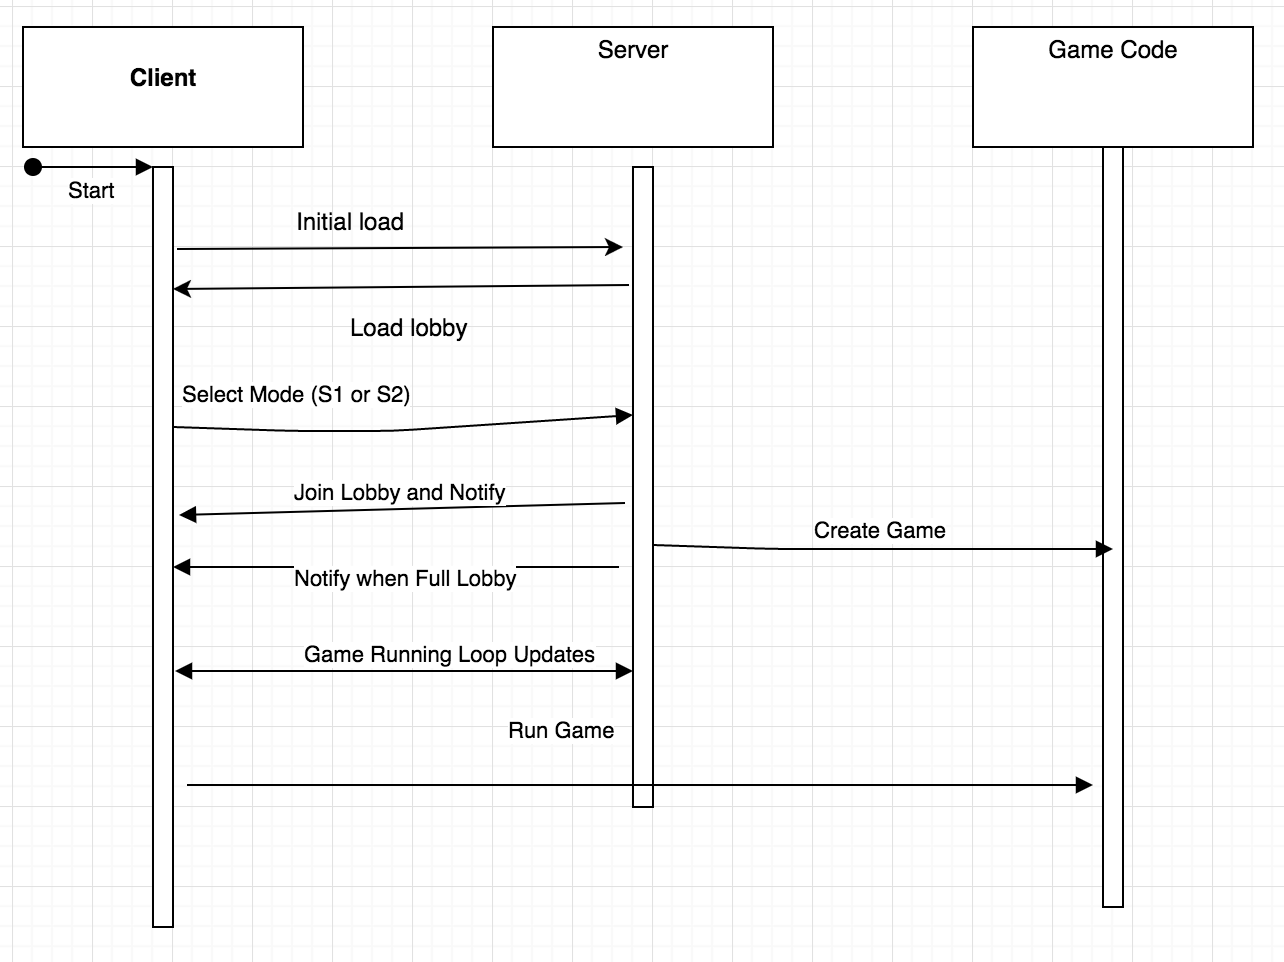
\includegraphics[width=\linewidth,height=7cm]{images/game_process.png}

\chapter{Contributions}

Shiranka Miskin:  did much of the initial work, developing the core of the application and implementing sufficient basic features to satisfy Deliverable 2.  Afterwards, he worked on researching and applying methods to mitigate latency effects on the client, as well as creating the map maker.  His code made up the Game Canvas, Client Controller, Mapper, as well as portions of the Server (\texttt{server/game-server.ts}), Game Logic (\texttt{core/game.ts}) and Main.  He also wrote the build process to compile and run the typescript application.\\

Sam Maier: focused primarily on backend work. He implemented the lobby code, deployed the application, and invested a lot of time on getting multi-process to work (which, in the end, it didn't). The majority of the code in src/server was written by him. \\

Addison Keizer: primarily worked on developing the code in the core game functionality. He built the Event system and interactions between objects, worked on adding entities like Walls and Bullets and contributed significantly to the rest of the core files. He also spent time developing the initial architecture designs. He spent significant time on the documents to submit. \\

Dhruv Lal: Dhruv Lal: He primarily worked on the client side functionality of the game as well as the functionality to determine when the game is supposed to be finished. He created the user interface for all of the non-gameplay screens (the main menu, lobby and game over screens). He also contributed a significant amount to the documents for each deliverable. \\



\end{document}
